
\section{Introduction}
Query logs allow us to bridge the theory and practice of SPARQL ~\cite{MartensT19}. These query logs ensure that the research conducted by the community is guided by the requirements and trends that emerge in practice.
The real-world SPARQL queries that are collected from public SPARQL endpoints have multiple use-cases such as performance evaluation in real-world settings, improve caching of triplestores, analysis on SPARQL adoption, query optimization, and usability analysis etc. \cite{stadleralsq}. The query logs produced by different SPARQL endpoints use different formats to syntactically represent records. In this work we consider Web Log Format and CSV. Within each format, the set of available fields -- the schemas -- vary. For example, the formats used by wikidata, bio2rdf, and virtuoso instances in default configuration are different schema variants of the Web Log Format~\cite{stadleralsq, SaleemAHMN15}.
%JSON etc
%In addition, these query logs often have formatting issues, making it difficult for a parser to extract required information from these logs. 
Furthermore, in order to utilize real-world SPARQL queries in the aforementioned use-cases, it is required to parse these queries and annotate them with various structural and data-driven features such number of triple patterns, list of projection variables used, the different types of joins used, the results size etc. Finally, annotating SPARQL queries in existing query logs needs a scalable processing engine. For example, DBpedia public SPARQL endpoint receives more than 100k queries everyday. Similarly, the Wikidata public endpoint receives thousands of queries on daily bases. 

To the best of our knowledge, there exist no generic and scalable software framework that parses these query logs to extract SPARQL queries, annotate them with different information, and convert them into an RDF dataset. 
To fill this research gap, we present the LSQ framework, which converts
SPARQL query logs into RDF dataset and attach various structural and data-driven features to each SPARQL query. In order to perform scalable RDF conversion, we make use of the Apache Spark Big Data framework. By default, the framework supports query logs from nine different formats. Support for other logs formats can be easily done by adding log patterns into the configuration file.  

This framework has already been used to convert query
logs of 27 public SPARQL endpoints from various public SPARQL endpoints such as DBpedia, Wikidata, Bio2RDF, Semantic Web Dog Food etc. The resulting RDF datasets are named as LSQ V2.0 \cite{stadleralsq}. The LSQ V2.0 represents 43.95 million executions of 11.56 million unique SPARQL queries, resulting in 1.24 billion triples.  
The LSQ queries have been used in many use cases such as benchmarking based on real-world SPARQL queries \cite{SaleemMN15,SaleemMSLN18,saleem2018largerdfbench,SaleemSCBMN19,hernandez2016querying,fernandez2019evaluating,azzam2020smart,bigerl2020tentris,AzzamAMKPH21,davoudian2021workload,9364498,9364380}, analysis of the SPARQL adoption in different applications \cite{han2016statistical,BonifatiMT17,bonifati2018darql}, improving caching strategies for SPARQL engines \cite{knuth2016scheduling,akhtar2018change,akhtar2019dynamic,SalasH18,safavi2019personalized}, useability analysis of the SPARQL \cite{arenas2016reverse,benedetti2016model,dellal2017addressing,stegemann2017investigating,Viswanathan18,Potoniec19,wang2019answering,BonifatiMT20,jian2020sparql,zhang2020revealing,ALMENDROSJIMENEZ2021113772,wang2021explaining}, and SPARQL query optimization \cite{song2016efficient,MartensT18,cheng2019opt+,FigueiraGKMNT20}. Since the initial release of the LSQ V1.0 \cite{SaleemAHMN15}, the datasets converted by our framework have been used in more than 50 research papers\cite{stadleralsq}. The scalable components developed into the LSQ framework have also contributed to the recent Apache Jena 4.6.0 release with additional improvements pending\footnote{For details please see: https://github.com/apache/jena/pull/712, 
https://github.com/apache/jena/pull/1475,
https://github.com/apache/jena/pull/1394, 
https://github.com/apache/jena/pull/1390, 
https://github.com/apache/jena/issues/1470, https://issues.apache.org/jira/projects/JENA/issues/JENA-2309}. 

The rest of the paper is organized as follows. In section 2, we present the LSQ framework. Section 3 discusses various use-cases where the datasets produced by our framework have already been used. In section 4, we present the useability instruction of this framework, followed by the availability information and sustainability plans in section 5. Finally, we conclude in section 6. 

\section{The LSQ Framework}
\begin{figure*}
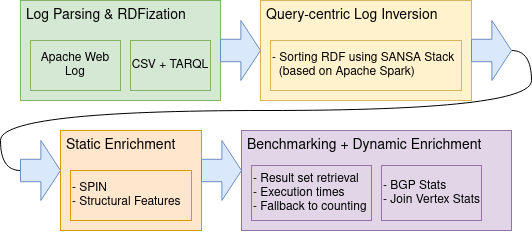
\includegraphics[width=\textwidth]{images/lsq2-architecture-new}
\caption{LSQ Framework Architecture. The underlying Semantic Web framework is Apache Jena.}
\label{fig:architecture}
\end{figure*}
In this section, we first briefly explain the core architecture. The details of each component is explained later. 

\Cref{fig:architecture} shows the architecture of LSQ which is briefly summarized as follows.
Records of query logs in different formats and having different schemas are parsed and normalized as RDF. 
The RDF log is inverted such that every query is related to all log records that mention it, i.e., every query is assigned a global (w.r.t, all query logs from different endpoints) identifier. 
In this process, queries are represented by hashes computed with their normalized strings. Static enrichment basically extracts the static features (that can be directly derived from a SPARQL query without running it against a specific RDF dataset) relevant to SPARQL query. It extends the RDF model with a SPIN\footnote{SPARQL SPIN representation: \url{https://www.w3.org/Submission/spin-sparql/}} and further static structural features such as the number of projection variables, number of triple patterns, join types and selectivities, the used syntactic elements (e.g. UNION, OPTIONAL) etc. %Furthermore, LSQ captures information about basic graph patterns (BGPs) which do not have a direct representation in the SPIN model. 
The dynamic enrichment extracts data-driven SPARQL features such as query runtime, result size or triple pattern selectivities etc.  Whereas static enrichment is independent on any dataset, dynamic enrichment needs a dataset as input. Benchmarking is a form of dynamic enrichment that extends a query's RDF model w.r.t. a dataset with result set sizes and execution times.
In the following, we present these steps in detail and how
%LSQ conceptual contributions as well as how
LSQ inspired creation of certain components which we contributed to other frameworks in order to facilitate reuse.
% something like: and how lsq makes conceptual contributions and how contributions to other frameworks were inspired by lsq



\subsection{Named Graph Stream Processing}
A fundamental design principle that is followed throughout LSQ is the \emph{entity graph} paradigm, also referred to as (named-)graph-per-entity:
An entity is represented by an IRI that appears in a (subject position of) triple in a named graph with the same IRI, such as \texttt{GRAPH :anEntity \{ :anEntity :p :o \}}.
Some Semantic Web tools (such as Virtuoso and Apache Jena) already support the use of named graphs with \texttt{CONSTRUCT} queries due to popular demand\footnote{\url{https://github.com/w3c/sparql-12/issues/31}}, although this feature is not part of the current SPARQL specification v1.1\footnote{\url{https://www.w3.org/TR/sparql11-query/}}.
LSQ uses the entity graph approach for representing log records and SPARQL queries.
The advantage of this approach are:
\begin{itemize}
\item The graph name acts as a natural entry point for starting exploration/traversals of the contained data. This is a convention applications (such as viewers) can support without having to rely on a specific (ad-hoc) vocabulary.
\item Retrieval and removal of all triples related to an entity is a simple operation on the named graph. This is of particular importance as certain models (e.g. SPIN) allow for arbitrary deeply nested tree structures in RDF which are extremely hard to query without scoping by a named graph.
\item Partitioning the data into self-contained named graphs is well aligned with the map-reduce paradigm: Operations on individual entities, such as enrichment operations, can be carried out naturally in parallel over a set of entity graphs using conventional Big Data frameworks. We created the necessary hadoop-based parsers as part of LSQ and contributed them to the SANSA stack (see \Cref{sec:sansa}).
\item An operation on an individual entity typically only requires its graph to be loaded rather than requiring access to \emph{all} triples across all entities, which allows for stream-processing with low memory usage.
\end{itemize}


% design issue that needed resolution was how to represent the information extracted from SPARQL queries.
%Initially, each logged query was directly transformed to RDF triples. However, this made it impossible to later extract retrieve all triples related to a specific
%query: The RDF model\todo{figure} of a query contains data along quite long paths. Furthermore, the spin model can represent arbitrarily nested RDF graphs.
%For this reason, the design choice was to use a \emph{graph-per-entity} approach 

\subsection{Parsing Query Logs}
Generally, LSQ parses query logs and transforms them into a set of named graphs of which each represents an individual log record. This means that every log file is harmonized to a common RDF model.

Query logs come in different formats, and within a format there can be many different schemas. By schema we refer to the set of available attributes per log record.
Manually determining the format and schema of a log is a very tedious task.
For this reason, LSQ features a log format registry which can be used to probe log files against.
Currently 2 types of log formats are supported: Web access log formats that are compatible with Apache HTTP server's mod\_log\_config\footnote{\url{https://httpd.apache.org/docs/current/mod/mod_log_config.html}}
and CSV. For the former, LSQ provides a custom mapping of log fields to an RDF model, for the latter a tarql-based\footnote{\url{https://github.com/tarql/tarql}} approach is supported where columns of the input file are mapped to RDF using a SPARQL construct query. Support for additional mapping languages, such as RML~\cite{dimou2014rml} or YARRML~\cite{Heyvaert2018Declarative} is future work. Note, that for the task of RDFizing a single CSV file, the practical difference between the approaches lies in syntax rather than functionality.

An excerpt of LSQ's log format registry configuration is shown in \Cref{lst:log-fmt-registry}.
So far the default registry comprises 10 formats/schema combinations.


\begin{lstlisting}[label=lst:log-fmt-registry, caption=RDF-based log format registry used in LSQ, style=lst, language=ttl, float=*, numbers=left]
fmt:combined
  a lsq:WebAccessLogFormat ;
  lsq:pattern "%h %l %u %t \"%r\" %>s %b \"%{Referer}i\" \"%{User-agent}i\"" .

fmt:bio2rdfProcessedCsv
  a lsq:CsvLogFormat ;
  lsq:pattern
"""
PREFIX lsq: <http://lsq.aksw.org/vocab#>
PREFIX prov: <http://www.w3.org/ns/prov#>
PREFIX xsd: <http://www.w3.org/2001/XMLSchema#>
CONSTRUCT {
  GRAPH ?s {
    ?s
      lsq:query ?query ;
      lsq:host ?domain ;
      lsq:headers [ <http://example.org/header#User-agent> ?agent ] ;
      prov:atTime ?t
  }
} {
  BIND(IRI(CONCAT('urn:lsq:', MD5(CONCAT(?query, '-', ?domain, '-', ?timestamp)))) AS ?s)
  BIND(STRDT(?timestamp, xsd:dateTime) AS ?t)
}
""" .
\end{lstlisting}



\subsection{Accessing RDF graphs via Object Models}

\begin{figure*}
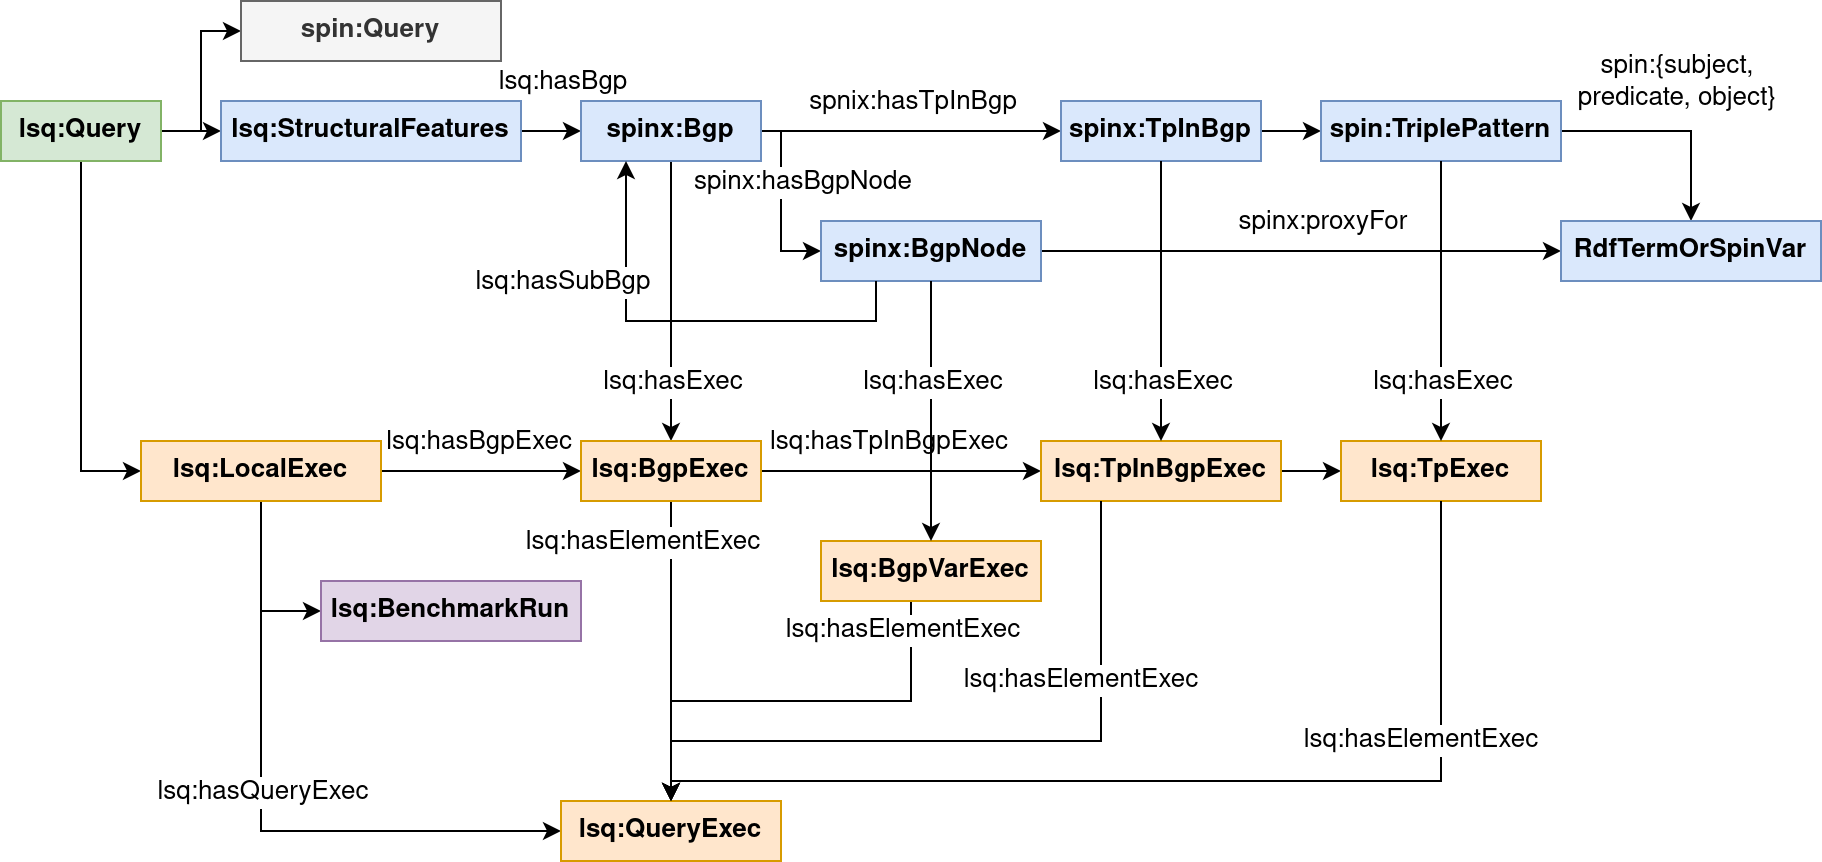
\includegraphics[width=\textwidth]{images/lsq2-datamodel-color-large}
\caption{LSQ2 Data Model}
\label{fig:datamodel}
\end{figure*}

The LSQ data model (see \Cref{fig:datamodel}) is sufficiently complex such that manipulation solely
with SPARQL turned out to be infeasible. One of the main reasons is due to the redundancy of complex graph patterns: Many patterns have to be repeated over and over again in different queries in order to address the nested resources. %which enrich.
Especially during development, any change in the T-box requires a change in several places and debugging SPARQL queries that yield empty result sets is a tedious process. Furthermore, deterministic skolemization of the model is an important aspect: We strictly want to avoid effects such as a merge of a query's RDF resulting in doubling the number of related BGPs as would be the case if blank nodes were used. Therefore, we need a way to express how to compute the identity of entities, such as: the id of a triple pattern depends on the id of its subject, predicate and object components, the id of a BGP depends on the ids of the contained triple patterns (in order) and the id of a specific triple pattern in a BGP depends on that of the BGP and its own.
%in order to avoid incorrectly repeating information such as the set of BGPs that are present in the model.

For this purpose, LSQ features a domain model realized as Java interfaces which must extend from Jena's \texttt{Resource} interface. The essence is, that the auto-generated implementations for this domain model then provides a \emph{view} over the RDF graph; all state is kept in the RDF graph and any invocation of a ``setter'' method directly mutates the RDF graph whereas a ``getter'' method reads from it.
Annotations on these interfaces are used to describe how getters and setters relate to triples in the underlying RDF graph. We use \emph{Reprogen} (Resource Proxy Generator)\footnote{\url{https://github.com/Scaseco/jenax/tree/develop/jenax-reprogen-parent/jenax-reprogen-core}} to generate Java proxies that implement the intended behavior of the annotations.

In order to realize skolemization, we extended Reprogen with new \texttt{@HashId} and \texttt{@StringId} annotations.
@HashIds are a way to control how to compute hash codes for an RDF term in an RDF graph w.r.t. to the annotated interface.
%If a method whose return value is neither a blank node nor IRI is annotated with @HashId then that value corresponds to a node at the boundary of a CBD. Hashes are computed for these literal values directly.
The hash code of a resource is obtained by recursively considering the hash codes of all its member methods annotated with \texttt{@HashId}.
The \texttt{@StringId} annotation is used for methods that can convert hash codes to strings suitable for use in IRIs.
%\Cref{lst:reprogen} shows an example for how to annotate a class whereas~\Cref{lst:reprogen-skolem} shows how to programmatically generate the corresponding RDF.
\Cref{lst:reprogen-skolem} shows how to programmatically generate RDF for an annotated class whereas
\Cref{lst:reprogen} shows an example for how to annotate a class.

%Otherwise, the HashId computation traverses along IRIs or blank nodes until non-resource attributes are encountered. %Hashes are the computed by performing a depth-first traversal to the boundary of the CDB,

\begin{lstlisting}[label=lst:reprogen-skolem, language=java, caption=Example for setting up and skolemizing a basic LSQ RDF model, style=lst, language=java, numbers=left]
Model model = ModelFactory.createModel();
LsqTriplePattern tp = model.createResource(LsqTriplePattern.class);
TpInBgp tpInBgp = model.createResource(TpInBgp.class);
tp.setJenaTriple(new Triple());

Resource root = Reprogen.skolemize(tpInBgp, "http://lsq.aksw.org");
RDFDataMgr.write(System.out, root.getModel(), RDFFormat.TURTLE_PRETTY);
\end{lstlisting}


\begin{lstlisting}[label=lst:reprogen, language=java, caption=Example of LSQ's annotated Java domain model for which Reprogen generates proxy implementations that can read and write to an RDF graph, style=lst, language=java, float=*, numbers=left]
/* The identity of a bgp depends on the list of identities of the contained
 * triple patterns */
public interface Bgp
 extends Resource
{
  @HashId
  @Iri(LsqTerms.hasTp)
  List<LsqTriplePattern> getTriplePatterns();
}

/* The identity of a "triple pattern in a bgp" depedends on the identity of
 * the bgp and the identity of the triple pattern */
public interface TpInBgp
  extends Resource
{
    @HashId
    @Iri(LsqTerms.hasBgp)
    SpinBgp getBgp();
    TpInBgp setBgp(Resource bgp);

    @HashId
    @Iri(LsqTerms.hasTp)
    LsqTriplePattern getTriplePattern();
    TpInBgp setTriplePattern(Resource tp);
}

\end{lstlisting}


%Maintaining skolemization in SPARQL queries using e.g. \texttt{BIND(IRI(CONCAT(STR(?baseIri), %'/aspect) AS ?aspect)} became infeasible.
%The requirements are as follows:
%\begin{itemize}
%\item A means to navigate a query's RDF model from LSQ's host language (Java).
%\item A mechanism to annotate which properties of a resource contribute to that resource's %identity.
%\end{itemize}


\subsection{Query Id Generation}
An important requirement in LSQ is determinism: Syntactically equivalent queries and their elements should always be represented by the same IRIs. The goal is to allow for the integration of different datasets generated by the same version of LSQ simply by means of merging the RDF.
Generally, query strings are normalized using a parse/string serialization round trip.
Query strings themselves are not suitable as identifiers because they can become very lengthy.
The obvious choice is thus to resort to hashing. LSQ v1 used 8 characters of md5 hashes however it turned out that the number of queries was sufficiently large that collisions occurred.
LSQ v2.0 uses sha256 with base64 encoding of the whole query string. The disadvantage was,
that queries that only differed in projection or slice received unrelated hashes. As a consequence, identifying queries that only differ in their 'basic parameterization' was not possible from the hashes.
LSQ v2.1 introduces additional structure:
The \emph{body hash} of a query is obtained by replacing the projection with 'SELECT *' and applying sha256+base64 hashing on the normalized query string.
A separate hash is computed from the projection: 
The actual projection expression strings are first sorted lexicographically and a projection-base-hash is computed from these ordered strings. The actual projection is then permutation of the sorted one, and numbering schemes exist to label permutations:
We use the \emph{Lehmer-Code} to obtain a number for the actual projection.
For a given sequence of $n$ items, the Lehmer-Code is 0 when that sequence is sorted and the code reaches its maximum value $n!$ when the sequence is reverse-sorted.

Finally, the slice is appended which leads to the new improved pattern
\texttt{bodyHash/projBaseHash/lehmerCode[/offset[-limit]]}.

%We number permutations on the basis of the \emph{Lehmer-Code}.
%We capture permutations of the projections by computing a number for the permutation on the basis of the \emph{Lehmer-Code}.

\subsection{LSQ Command Line Interface}
In this section we briefly present the workflow for benchmarking a SPARQL endpoint with the
\texttt{lsq} command line tool.

%In a first step, an RDF model of the query log .
%Log records are 

LSQ aims to capture on which endpoint a query was executed at which point in time.
For that purpose, LSQ can reuse timestamps in log files. If such are absent then sequential numbering is used as a fallback. The URL of the endpoint from which a query log file originated needs to be provided manually.
%externally.
The endpoint for RDFization is purely of informational nature. No requests will be made to it. In principle, if it was known which dataset was available at an endpoint at a certain point in time, then this information can be used to link to a dataset identifier. Furthermore, ideally a dataset identifier can be linked to a download URL of exactly the set of RDF triples (or quads) that were present at that endpoint. Although this background knowledge is currently usually not systematically available, we envision this situation to improve with advancements in data catalog and service modeling such as with DCAT\footnote{\url{https://www.w3.org/TR/vocab-dcat-2/}}.
An example of a command line invocation and its corresponding output is shown in~\Cref{lst:lsq-rdfize} and~\Cref{lst:lsq-rdfize-output}.
\begin{lstlisting}[label=lst:lsq-rdfize, caption={Command for rdfizing a SPARQL query log}, style=lst, language=bash, numbers=left]
lsq rx rdfize --endpoint=http://dbpedia.org/sparql virtuoso.dbpedia.log 
\end{lstlisting}

\begin{lstlisting}[label=lst:lsq-rdfize-output, caption={The output of the rdfization is one named graph per query}, style=lst, language=ttl, numbers=left]
:lsqQuery-X {
  :lsqQuery-X
    lsq:text "SELECT * { ?s ?p ?o }" ;
    lsq:hasRemoteExec :remoteExec-org-dbpedia-sparql_2016-04-10T01:00:00Z .

  :remoteExec-org-dbpedia-sparql_2016-04-10T01:00:00Z
    lsq:endpoint <http://dbpedia.org/sparql> ;
    prov:atTime "2016-04-10T01:00:00Z"^^xsd:dateTime .
}
:lsqQuery-Y { ... }
\end{lstlisting}

Note, that the output is query-centric, which means that the input sequence of records is sorted by the query hash. The \texttt{rx} variant uses linux sorting which is not portable, whereas \texttt{spark} variant provides a portable java-native solution.

\subsection{Benchmarking}
LSQ uses RDF to keep benchmark settings in order to relate benchmark results to the context under which they were obtained.
For this reason, benchmarking is a three step process: (1) Create a \emph{benchmark configuration}. This is an RDF document which contains an IRI that carries the settings. The IRI is described with the date when the configuration was created and a custom label. The latter is useful for organization because benchmarking is often performed against SPARQL endpoints under a localhost URL from which no expressive name can be derived. Benchmark creation also caches the number of triples in the endpoint with the configuration. This number is used to compute certain ratios, such as the ratio of triples matched by a single triple pattern w.r.t. to the total size of the RDF graph.
As a consequence, a new configuration should be created whenever the settings or the data changes.
(2) Prepare a \emph{benchmark run}: This is another little RDF document which only introduces an IRI with two pieces of information: The IRI of the configuration and the timestamp of when the run was prepared.
(3) Execute the benchmark. Every benchmark task will be linked to the IRI of the benchmark run which in turn links to the used configuration.
\Cref{lst:lsq-cli-benchmark} demonstrates the command line invocations for setting up and running a benchmark whereas an example configuration is shown in~\Cref{lst:lsq-bench-conf}.

\begin{lstlisting}[label=lst:lsq-cli-benchmark, caption=Example benchmark setup and execution, style=lst, language=bash, float=*]
lsq benchmark create --endpoint http://localhost:8080/sparql --dataset dbpedia
# Assumed output: xc-dbpedia_2021-10-22.conf.ttl
lsq benchmark prepare -c xc-dbpedia_2021-10-22.conf.ttl
# Assumed output: c-dbpedia_2021-10-22_2021-10-22T12_26_40_828056Z.run.ttl
lsq benchmark run -c xc-dbpedia_2021-10-22_2021-10-22T12_26_40_828056Z.run.ttl virtuoso.dbpedia.trig
\end{lstlisting}

\begin{lstlisting}[label=lst:lsq-bench-conf, caption=Excerpt of benchmark configuration options, style=lst, language=ttl, float=*, numbers=left]
lsqr:xc-dbpedia_2021-10-22
        dct:identifier                  "xc-dbpedia_2021-10-22" ;
        lsqo:connectionTimeoutForRetrieval  "60"^^xsd:decimal ;
        lsqo:executionTimeoutForRetrieval  "300"^^xsd:decimal ;
        lsqo:maxResultCountForRetrieval  "1000000"^^xsd:long ;
        lsqo:maxByteSizeForRetrieval    "-1"^^xsd:long ;
        lsqo:maxResultCountForSerialization  "-1"^^xsd:long ;
        lsqo:maxByteSizeForSerialization  "1000000"^^xsd:long ;
        lsqo:executionTimeoutForCounting  "300"^^xsd:decimal ;
        lsqo:connectionTimeoutForCounting  "60"^^xsd:decimal ;
        lsqo:benchmarkSecondaryQueries  true .
\end{lstlisting}
\subsubsection{Benchmark Workflow}
When benchmarking a query, an IRI is allocated based on the benchmark run id and the query id.
Within an individual benchmark run a query can only be executed once. A database (TDB2) is used to keep track of query hashes that have already been benchmarked.
LSQ first attempts to benchmark and retrieve the result set of a query. 
If retrieval succeeds (and no thresholds are exceeded) then the retrieved result set is serialized as a literal in the output RDF dataset as long as the serialization thresholds are adhered to.
If the retrieval fails due to threshold violation (in contrast to e.g. a syntactic error) then an alternate strategy is employed which attempts to count the size of the query by wrapping it with \texttt{SELECT (COUNT(*) AS ?c) \{ ... \}}. The benchmark result contains triples for any exceeded thresholds.
%In principle, this could be modeled as the benchmark result of the count-query, however to 

\paragraph{Benchmarking Secondary Queries} Primary queries are those originating from a query log. Secondary queries are those derived from the syntactic elements of primary ones. The most prominent elements are basic graph patterns and individual triple patterns. A secondary query is benchmarked just like a primary one. The rule that a query will only be benchmarked once within a run thus also applies.


An example RDF representation of a SPARQL query generated by the LSQ framework is shown in Listing \ref{lst:reprsentation}. We encourage authors to have a look at LSQ V2.0 paper \cite{stadleralsq} for further details of the RDF representation.  

\begin{lstlisting}[caption = {An example LSQ/RDF representation of a SPARQL query in Turtle syntax \cite{stadleralsq}},label = {lst:reprsentation},style=lst,basicstyle={\scriptsize\ttfamily},language=ttl,frame={single},breaklines=true,stepnumber=1,float=*, numbers=left]
@prefix rdf:	<http://www.w3.org/1999/02/22-rdf-syntax-ns#> .
@prefix lsqr:	<http://lsq.aksw.org/> .
@prefix lsqv:	<http://lsq.aksw.org/vocab#> .
@prefix rdfs:	<http://www.w3.org/2000/01/rdf-schema#> .
@prefix swc:	<http://data.semanticweb.org/ns/swc/ontology#> .
@prefix swr:	<http://data.semanticweb.org/> .
@prefix xsd:	<http://www.w3.org/2001/XMLSchema#> .
@prefix prov:	<http://www.w3.org/ns/prov#> .

# Primary resource describing the query found with the SWDF logs
lsqr:lsqQuery-3wBd2uKotB_-vUxnngs6ZNsGPhJmIDD9c7ig0UI24y8	
	lsqv:hasLocalExec lsqr:localExec-v9fBp3ElS1aVXXN1Z8zX1jxcHX3iy-axTgRrU2c7NY8 ;
	lsqv:hasRemoteExec lsqr:re-data.semanticweb.org-sparql_2014-05-22T16:08:17Z ,
		lsqr:re-data.semanticweb.org-sparql_2014-05-20T13:24:13Z ;
	lsqv:hasStructuralFeatures lsqr:lsqQuery-3wBd2uKotB_-vUxnngs6ZNsGPhJmIDD9c7ig0UI24y8-sf ;
	lsqv:hash "3wBd2uKotB_-vUxnngs6ZNsGPhJmIDD9c7ig0UI24y8" ;
	lsqv:text """PREFIX  rdf:  <http://www.w3.org/1999/02/22-rdf-syntax-ns#>
	               PREFIX  swc:  <http://data.semanticweb.org/ns/swc/ontology#>
	               SELECT DISTINCT  ?prop
	               WHERE { ?obj  rdf:type swc:SessionEvent ; ?prop ?targetObj FILTER isLiteral(?targetObj)  }
	               LIMIT   150""" .

# Static features of the query
lsqr:lsqQuery-3wBd2uKotB_-vUxnngs6ZNsGPhJmIDD9c7ig0UI24y8-sf	
	lsqv:bgpCount 1 ;
	lsqv:hasBgp lsqr:bgp-_x9Mckke-V9R3ddISuw-Nj_j278nT5HwiA1WUNk7tgY ;
	lsqv:joinVertexCount 1 ;
	lsqv:joinVertexDegreeMean 2 ;
	lsqv:joinVertexDegreeMedian 2 ;
	lsqv:projectVarCount 1 ;
	lsqv:tpCount 2 ;
	lsqv:tpInBgpCountMax 2 ;
	lsqv:tpInBgpCountMean 2 ;
	lsqv:tpInBgpCountMedian 2 ;
	lsqv:tpInBgpCountMin 2 ;
	lsqv:usesFeature lsqv:fn-isLiteral , lsqv:Select , lsqv:Limit , lsqv:Functions , lsqv:Group , lsqv:Filter , 
		lsqv:Distinct , lsqv:TriplePattern .              

# Remote execution no. 1 on the original endpoint
lsqr:re-data.semanticweb.org-sparql_2014-05-22T16:08:17Z	
	prov:atTime "2014-05-22T16:08:17Z"^^xsd:dateTime ;
	lsqv:endpoint swr:sparql ;
	lsqv:hostHash "O5UQpDtofxAsrJk7yzGfDolFGylMFw5446KcRZDcBkU" .

# Remote execution no. 2 on the original endpoint
lsqr:re-data.semanticweb.org-sparql_2014-05-20T13:24:13Z	
	prov:atTime "2014-05-20T13:24:13Z"^^xsd:dateTime ;
	lsqv:endpoint swr:sparql ;
	lsqv:hostHash "7aPNvqsgizRuEjH7_cO_dXoqLk-exKJ-xFmbCH3ew_E" .

# Local execution to extract statistics
lsqr:localExec-v9fBp3ElS1aVXXN1Z8zX1jxcHX3iy-axTgRrU2c7NY8-xc	
	lsqv:benchmarkRun lsqr:xc-swdf_2020-09-23_at_23-09-2020_17:10:19 ;
	lsqv:hasQueryExec lsqr:queryExec-Cmv7SccybbBxwkep_cHvDiF3piq29tH7NWlDfIiCHqU .

# Results of local execution
lsqr:queryExec-Cmv7SccybbBxwkep_cHvDiF3piq29tH7NWlDfIiCHqU	
	prov:atTime "2020-09-23T15:27:36.325Z"^^xsd:dateTime ;
	lsqv:countingDuration 0.008466651 ;
	lsqv:evalDuration 0.008868635 ;
	lsqv:resultCount 16 .
		
# The full data further include a SPIN description of the query, a list of BGPs within the query,
# a list of triple patterns and terms within the query, as well as execution statistics for individual
# BGPs, triple patterns and sub-BGPs induced by join variables
\end{lstlisting}


\subsection{Scaling LSQ with SANSA}
\label{sec:sansa}
Processing large log files with only a single core is tedious and anachronistic in times of Big Data and laptops having more than a dozen cores. Apache Spark is a framework that enables scaling computing tasks to use all available resources on a cluster -- even if the "cluster" only comprises a single machine. Apache Spark features high level abstractions for distributed executions of operations on different types of distributed collections of records. \emph{Resilient Distributed Datasets} (RDDs) are the ones used by LSQ/Spark.
However, the low-level I/O for reading records from files (regardless whether in local or distributed file systems) is provided by Apache Hadoop.
The now retired Apache Jena/Elephas\footnote{\url{https://jena.apache.org/documentation/archive/hadoop/}} project provided distributed ingestion of RDF data by wiring its own I/O library (called \emph{RIOT}) up with Apache Hadoop. However, while Elephas supported n-quads, this format is both much more verbose and more hard to read than pretty printed trig.
Conversely, manually reviewing rather sophisticated LSQ models in trig format was significantly easier, however, Elephas could not read trig in splits. Therefore use of this format negated the benefits of the Big Data framework.
In order to optimize processing, we created an initial distributed parser for trig that searched hadoop input splits by matching the \texttt{<graphname> \{ ... \}} pattern.
This framework was continuously extended to handle RDF prefixes and even RDF data in literals.
By now, this parsing framework has evolved into \emph{Hadoop Generic Parser Framework} (HGPF) and provides support for trig (a superset of turtle, n-quads and n-triples), JSON and CSV.

\Cref{lst:sansa-rdf} shows the contribution made to SANSA in order to enable processing of large trig files (of which n-quads is a special case) with LSQ. The parser has been successfully used to ingest and sort 500GB of LSQ trig data in about 5 hours on a 3 node spark cluster.
%\todo{This should be mentioned in an eval section}

\begin{lstlisting}[label=lst:sansa-rdf,language=java, caption=Parsing named graph streams, style=lst, language=java, numbers=left]
RdfSourceFactory rdfSourceFactory = RdfSourceFactoryImpl.from(sparkSession);
RdfSource rdfSource = rdfSourceFactory.get("query-log.lsq.trig");
RDD<Quad> rddOfQuads = rdfSource.asQuads();
RDD<DatasetOneNg> rddOfDataset = rdfSource.asDatasets();
\end{lstlisting}

The HGPF framework has also been used to realize a CSV parser that can also handle multi-line cell values. The limitation is that when searching for candidate record offsets in a split, the maximum size of multi-line cells needs to be configured in advance.
The default value is 500KB, and the candidate record offset detector always has to exhaust this amount of data in order not to miss any cell endings.

The CSV settings are based on the \emph{frictionless data csv dialect} which slightly extends
over the \emph{CSV on the Web} (CSVW)\footnote{\url{https://www.w3.org/TR/tabular-data-model/}} specification.
An example of programmatic usage is shown in~\Cref{lst:sansa-csv}.
\begin{lstlisting}[label=lst:sansa-csv,language=java, caption=Example for setting up and skolemizing a basic LSQ RDF model, style=lst, language=java, numbers=left]
JavaRDD<Binding> rddOfBindings = CsvDataSources.createRddOfBindings(sparkContext, "data.csv", csvDialect);
Query query = QueryFactory.create("CONSTRUCT ...");
JavaRDD<Quad> rddOfQuads = JavaRddOfBindingsOps.tarqlQuads(rddOfBindings, query);
\end{lstlisting}





\section{Impact}
To the best of our knowledge, the framework we propose in this paper is the first generic framework for RDFizing SPARQL query logs in different formats.
Furthermore, it does so in a scalable way by following Big Data processing paradigms.
There was no mechanism available to reuse existing query logs in a single standard format with much more enriched information attached to each query.
Our framework is completely abided by semantic web technologies.
It has been used to convert query logs of 27 public SPARQL endpoints, resulting in terabytes of RDF data.

In the recent LSQ v2.0 paper \cite{stadleralsq}, potential six use cases -- custom benchmarking, SPARQL adoption, caching, usability analysis, query optimisation, and meta-querying -- have been discussed.
The RDF datasets generated using the LSQ framework have been used widely for these use-cases \cite{stadleralsq}.
 he study \cite{stadleralsq} reported that 29 research papers have used LSQ queries for custom benchmarking, six  research papers for SPARQL adoption, five research papers for caching,
 12 research papers for SPARQL useability analysis, seven research papers for query optimisation, and two papers for meta-querying  \cite{stadleralsq}.
 Furthermore, \cite{stadleralsq} discussed a number of works which have used LSQ (mostly for evaluation) in contexts that were not originally anticipated by the aforementioned use cases.
 These works include predicting temporal relations between events \cite{georgala2016efficient}, augmenting RDF data sources with completeness statements~\cite{fafalios2019many},
 finding the frequency and distribution of answerable and non-answerable query patterns \cite{fafalios2019many}, question answering over linked data ~\cite{singh2019qaldgen},
 and a blockchain that allows users to propose updates to faulty or outdated data~\cite{AebeloeMH21}. 

\section{Reusability}
We are hopeful that the LSQ framework will be used by more researchers to convert existing query logs and create LSQ datasets. The resource home page includes documentation along with examples for easy reusability. The components developed in the LSQ framework are very generic. A dockerized version of the LSQ is also available from the resource homepage. The LSQ framework can also be adopted to other log formats by providing the log pattern, e.g., CSV, specific text pattern. Custom enrichment can also be done, i.e, add more query features attached to each query. The resource homepage includes a wiki explaining how others can use the framework along with examples and CLI instructions. So far, we have not tested the framework with XML, JSON logs. However, it should be working provided that the correct log pattern is specified in the configuration file. 


\section{Availability and Sustainability}
The resource is available from a persistent URL \url{http://w3id.org/lsq}. LSQ v2.0 \cite{stadleralsq} is the canonical citation associated with this resource. Our framework and LSQ datasets are available under GNU General Public License v3.0. The source code is publicly available via Github. 
All future extensions will be reflected on the same persistent URL. In addition, this framework will be sustained via the Paderborn Center for Parallel Computing $PC^2$, which provides computing resources as well as consulting regarding their usage to research projects at Paderborn University and also to external research groups. The Information and Media Technologies Centre (IMT) at Paderborn University also provides a permanent IT infrastructure to host the LSQ project.

\section{Conclusion}
In this paper, we have presented the LSQ framework, a scalable engine to represent queries in logs as RDF, allowing users perform their analysis on real-world SPARQL queries. We discussed the core architecture of this software framework along with potential impact and the useability instructions. We briefly discussed various use-cases where RDF datasets produced by our framework have already been used. In the future, we want to further extend this framework that provides further annotated information, e.g. annotating the named entities used in the SPARQL queries and their disambiguation to well-known datasets such Wikidata and DBpedia. We aim to collect further query logs from public SPARQL endpoints and provide them as RDF datasets. 




\paragraph*{Resource Availability Statement:}\label{resource} \begin{itemize}
    \item Source code of the LSQ framework is available from \url{https://github.com/AKSW/LSQ}
    \item Installation instructions available from \url{http://lsq.aksw.org/v2/setup.html}
    \item Usage instructions available from \url{http://lsq.aksw.org/v2/usage/usage.html}
    \item RDF dumps of the LSQ v2.0 datasets available from \url{https://hobbitdata.informatik.uni-leipzig.de/lsqv2/dumps/}
    \item LSQ V2.0 public SPARQL endpoint is available from \url{http://lsq.aksw.org/sparql}
    \item Set of useful SPARQL queries over LSQ datasets available from \url{http://lsq.aksw.org/v2/usage/usage.html}

    \item The resource type is Software Framework
 and is available under GNU General Public License v3.0

    \item All of the above information along with legacy data and old LSQ maintenance information available from the resource persistent URL \url{http://w3id.org/lsq}
    \item LSQ V2.0 \cite{stadleralsq} is the canonical citation associated with this paper 
\end{itemize}




